An important measure of the robustness of a traffic rule is its ability to resolve traffic disturbance. Here we adopt a hybrid of car-following and classic kinematic wave theory from literature \cite{tang_2004}.  In this theory, classic LWR kinematcs wave model \cite{lighthill_1955,richards_1955} is combined with a variation of car-following theory \cite{jiang_2002}, giving the following four equations that describe the temperal and spatial variations of the traffic density as well as average velocity of vehicles on the two lanes of the freeway.
	\begin{align} \label{eq:pde}
	& \frac{\partial \rho_1}{\partial t} + \frac{\partial \rho_1}{\partial x}v_1+\rho_1\frac{\partial v_1}{\partial x}=s_1 & \\
	& \frac{\partial v_1}{\partial t} + v_1\frac{\partial v_1}{\partial x} = \frac{v_{1e}-v_1}{\tau_1}+c_{10}\frac{\partial v_1}{\partial x} & \\
	& \frac{\partial \rho_2}{\partial t} + \frac{\partial \rho_2}{\partial x}v_2+\rho_2\frac{\partial v_2}{\partial x}=s_2 & \\
	& \frac{\partial v_2}{\partial t} + v_2\frac{\partial v_2}{\partial x} = \frac{v_{2e}-v_2}{\tau_2}+c_{20}\frac{\partial v_2}{\partial x} &
	\end{align}
	where we take $v_{1e} = v_{2e}$ to be the equilibrium velocity-density relations derived from previous sections (equation (\ref{eq:ve})). Adhering to the assumption that the two roads are identical, we choose $\tau_1=\tau_2=10s$ and $c_{10}=c_{20}=11m/s$ according to the stability contraint proposed by Tang and Huang\citep{tang_2004}.
	
	We impose periodic boundary condition and initial condition that represents a traffic disturbance in lane 1 to observe traffic behavior after the disturbance. $\rho_1(x,0)$ is the functional form of a traffic disturbance suggested in \citep{tang_2004}. $L$ is the length of freeway of interest. $\rho_{10}$ is the average vehicle density on lane 1 and $\Delta \rho_{10}$ is the size of the disturbance. 
	\begin{align}
	& \rho_1(0,t) = \rho_1(L,t) & \\
	& v_1(0,t) = v_1(L,t) & \\
	& \rho_2(0,t) = \rho_2(L,t) & \\
	& v_2(0,t) = v_2(L,t) & \\
	&\rho_1(x,0)=\rho_{10}+\Delta \rho_{10}\left(  cosh^{-2}(\frac{160}{L}(x-\frac{5L}{16}))-\frac{1}{4}cosh^{-2}(\frac{40}{L}(x-\frac{11L}{32})) \right)& \\
	& v_1(x,0) = v_{1e}(\rho_1(x,0)) & \\
	&\rho_2(x,0)= \rho_{20}& \\ \label{eq:ic}
	& v_2(x,0) = v_{2e}(\rho_2(x,0)) & \\
	\end{align}
	
	The source terms for lane 1 and lane 2 must satiesfy  $s_1+s_2=0$ by the assumption of no on/off ramp. By changing these source terms, we are effectively putting different traffic rules into effect. For example, $s_1=0$ correspond to the rule that no vehicle is allowed to switch lanes, whereas $s_1= \rho_2-\rho_1$ enforces the rule that vehicles are only allowed to switch from lane 1 to lane 2 if the car density on lane 2 is lower than that on lane 1. Here we adopt the rule $s_1=\rho_2/\rho_{20}-\rho_1/\rho_{10}$. The addition of $\rho_{10}$ and $\rho_{20}$, the equilibrium densities for the two lanes, allows us to bias the utilization of the two roads. Specifically, if the keep-right rule is enforced (and suppose lane 2 is the overtaking lane), then vehicles on lane 2 must generally have faster speed than those on lane 1, therefore by the reciprocal velocity-density relation (equation \ref{eq:ve}) we can imply $\rho_{10}>\rho_{20}$.
		
	Recall that the equilibrium velocity-density relation (equation \ref{eq:ve}) produces a natural speed limit of $50$ m/s and a jaming density of $\rho_j=0.19$ cars/m. This provides us with a guideline for the overall scale of equilibrium traffic for light and heavy conditions. For the fair comparison, the total number of cars on the road is supposed to be the same for the case with no rule enforced and the case with the keep-right rule. For light traffic we chose $\rho_{10}+\rho_{20}=0.06 \approx \frac{1}{3}\rho_j$ whereas for heavy traffic we chose $\rho_{10}+\rho_{20}=0.24 \approx \frac{5}{4}\rho_j$
	Equations (\ref{eq:pde}-\ref{eq:ic}) are solved using Mathematica 9.0. Four sets of parameters were chosen to represent
	\begin{enumerate}
	\item{light traffic, no rule:}
		$\rho_{10}=\rho_{20}=0.03, \Delta \rho_{10}=0.001$
		\begin{figure}[h]
		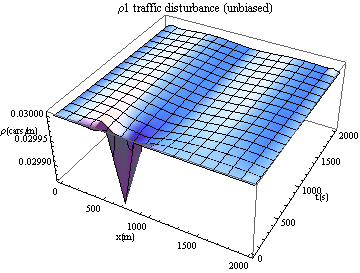
\includegraphics[scale=.6]{plot/p1_light_disturb_unbiased}
		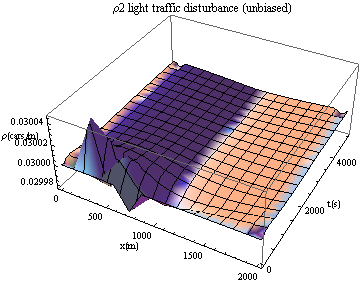
\includegraphics[scale=.6]{plot/p2_light_disturb_unbiased}
		\end{figure}
	\item{light traffic, keep-right:}
		$\rho_{10}=0.045, \rho_{20}=0.005, \Delta \rho_{10}=0.001$
		\begin{figure}[h]
		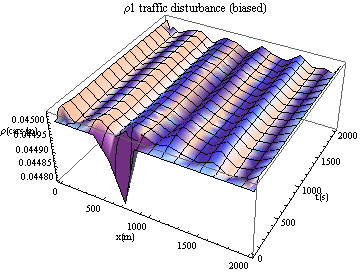
\includegraphics[scale=.6]{plot/p1_light_disturb_biased}
		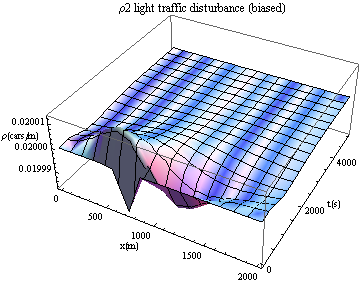
\includegraphics[scale=.6]{plot/p2_light_disturb_biased}
		\end{figure}
	\item{heavy traffic, no rule:}
		$\rho_{10}=\rho_{20}=0.12, \Delta \rho_{10}=0.001$
		\begin{figure}[h]
		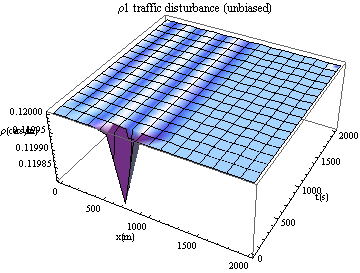
\includegraphics[scale=.6]{plot/p1_heavy_disturb_unbiased}
	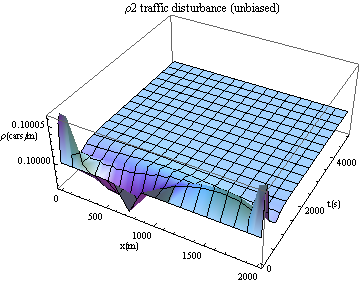
\includegraphics[scale=.6]{plot/p2_heavy_disturb_unbiased}
		\end{figure}
	\item{heavy traffic, keep-right:}
		$\rho_{10}=0.19, \rho_{20}=0.05, \Delta \rho_{10}=0.001$
		\begin{figure}[h]
		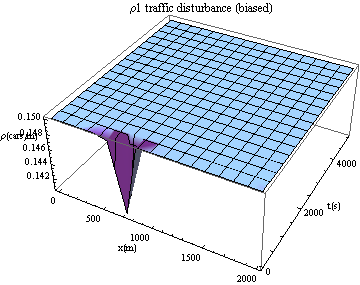
\includegraphics[scale=.6]{plot/p1_heavy_disturb_biased}
		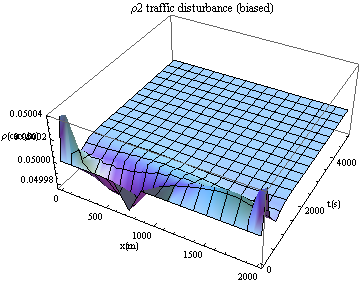
\includegraphics[scale=.6]{plot/p2_heavy_disturb_biased}
		\end{figure}
	\end{enumerate}
	Under light traffic conditions, having no rule actually helps the stability of traffic, a slight disturbance in one lane does not cuase lasting disturbance, whereas when the keep-right rule is enforced, lasting disturbance, even though very slight, will survive.	
	
	Under heavy traffic conditions, on the other hand, reverese the situation. Having the keep-right rule dramatically increases the stability of traffic against a slight disturbance.